\documentclass{beamer}
\usetheme{Madrid}
\usecolortheme{default}
\usepackage{listings}
\usepackage{tcolorbox}
\tcbuselibrary{listings, skins}

\newtcblisting{mycode}{
  arc=0mm,                          % Sharp corners
  boxrule=0.5pt,                    % Border thickness
  colback=white,                    % Background color
  colframe=black,                   % Border color
  listing only, 
  listing options={
    language=Python,
    basicstyle=\small\ttfamily,      % Monospace font
    keywordstyle=\color{blue},       % Color for 'import', etc.
    commentstyle=\color{blue},       % Color for comments
    stringstyle=\color{red},
    showstringspaces=false,
    breaklines=true
  },
  sharp corners,
  enhanced,
}

\title{Analog-1.1.27}
\author{INDHIRESH S-EE25BTECH11027}
\date{\today}

\begin{document}

\begin{frame}
    \titlepage
\end{frame}

\begin{frame}{Question}
Consider the op-amp circuit shown.
\begin{figure}[H]
    \centering
    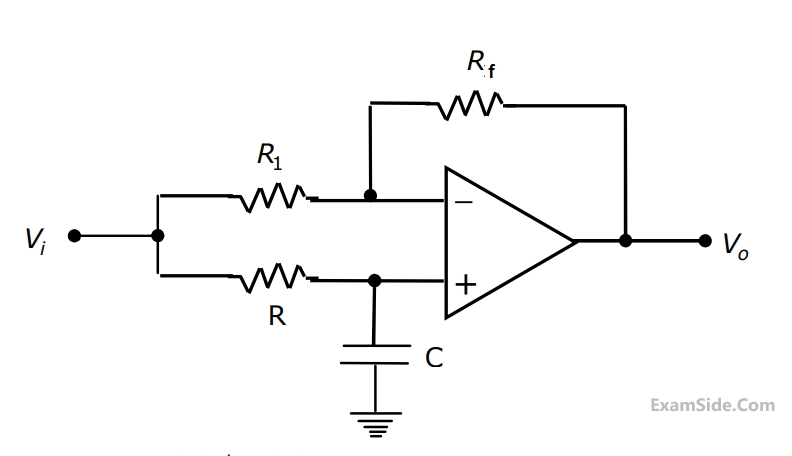
\includegraphics[width=0.4\linewidth]{ques.jpg}
    \caption{Op-amp circuit}
    \label{fig:placeholder}
\end{figure}
\begin{enumerate}

\item The transfer function Vo(s)/Vi(s) is:\\

\begin{columns}[t]
    \column{0.2\textwidth}
    1) $\frac{1-sRC}{1+sRC}$
    \column{0.2\textwidth}
    2) $\frac{1+sRC}{1-sRC}$
    \column{0.2\textwidth}
    3) $\frac{1}{1-sRC}$
    \column{0.2\textwidth}
    4) $\frac{1}{1+sRC}$
\end{columns}
\vspace{20pt}
\item If Vi = Vi sin($\omega$t) and Vo = Vo sin($\omega$t + $\phi$), the minimum and maximum values of $\phi$ (in radians) are respectively:
\begin{columns}[t]
    \column{0.2\textwidth}
    1)-$\frac{\pi}{2}$ and $\frac{\pi}{2}$
    \column{0.2\textwidth}
    2)0 and $\frac{\pi}{2}$
    \column{0.2\textwidth}
    3) -$\pi$ and 0
    \column{0.2\textwidth}
    4)-$\frac{\pi}{2}$ and 0
\end{columns}
\end{enumerate}
\end{frame}
\begin{frame}{Equivalent Circuit in s-domain}
\begin{figure}
    \centering
    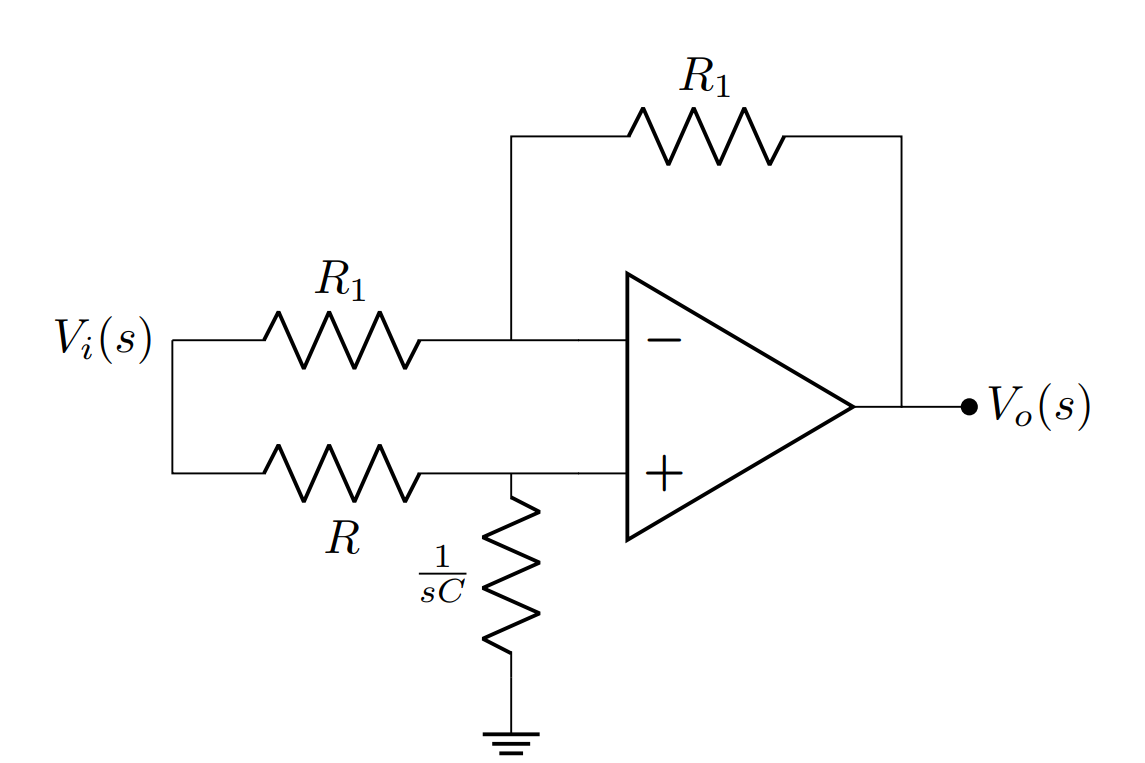
\includegraphics[width=\linewidth]{s domain ckt.png}
    \caption{Caption}
    \label{fig:placeholder}
\end{figure}
    
\end{frame}

\begin{frame}{ Analysis of the Non-Inverting Terminal}
    The input $v_i(t)$ is applied to the RC network connected to the non-inverting terminal ($v_+$).
    \par\vspace{0.3cm}
    Applying KCL at node $v_+$:
    $$\frac{v_i(t) - v_+(t)}{R} = C \frac{dv_+(t)}{dt}$$
    \par\vspace{0.3cm}
    Rearranging to form a standard RC differential equation:
    \begin{equation}
        v_i(t) = RC \frac{dv_+(t)}{dt} + v_+(t) \label{eq:vplus}
    \end{equation}
\end{frame}

\begin{frame}{Analysis of the Inverting Terminal}
    For an ideal op-amp, $v_- = v_+$. Applying KCL at the inverting terminal:
    $$\frac{v_i(t) - v_+(t)}{R_1} + \frac{v_o(t) - v_+(t)}{R_1} = 0$$
    \par\vspace{0.3cm}
    Since the $R_1$ resistors are equal, they cancel out:
    $$v_i(t) - v_+(t) + v_o(t) - v_+(t) = 0$$
    \par\vspace{0.3cm}
    Solving for $v_+(t)$:
    \begin{equation}
        v_+(t) = \frac{v_o(t) + v_i(t)}{2} \label{eq:vsub}
    \end{equation}
\end{frame}
\begin{frame}{Combining the Results}
    Substitute Equation (\ref{eq:vsub}) into Equation (\ref{eq:vplus}):
    $$v_i(t) = RC \frac{d}{dt} \left[ \frac{v_o(t) + v_i(t)}{2} \right] + \frac{v_o(t) + v_i(t)}{2}$$
    \par\vspace{0.3cm}
    Multiply the entire equation by 2 to clear the fraction:
    $$2v_i(t) = RC \frac{dv_o(t)}{dt} + RC \frac{dv_i(t)}{dt} + v_o(t) + v_i(t)$$
    \par\vspace{0.3cm}
    Group the input and output terms:
    $$RC \frac{dv_o(t)}{dt} + v_o(t) = v_i(t) - RC \frac{dv_i(t)}{dt}$$
\end{frame}


\begin{frame}{Final Differential Equation}
    The time-domain behavior of the first-order all-pass filter is governed by:
    \vfill
    \begin{block}{Final Result}
        $$RC \frac{dv_o(t)}{dt} + v_o(t) = v_i(t) - RC \frac{dv_i(t)}{dt}$$
    \end{block}
   
\end{frame}

\begin{frame}{Method 2: The Transform Domain Approach}
    If we already know the Transfer Function $H(s)$, we can derive the differential equation through the Inverse Laplace Transform.
    \par\vspace{0.3cm}
    The Transfer Function for this all-pass filter is:
    $$H(s) = \frac{V_o(s)}{V_i(s)} = \frac{1 - sRC}{1 + sRC}$$
    \par\vspace{0.3cm}
    Cross-multiplying the terms gives:
    $$V_o(s)(1 + sRC) = V_i(s)(1 - sRC)$$
    \par\vspace{0.3cm}
    Expanding both sides:
    $$V_o(s) + sRC V_o(s) = V_i(s) - sRC V_i(s)$$
\end{frame}

% Slide: Inverse Laplace Transformation
\begin{frame}{ Applying Inverse Laplace Transform}
    Using the Laplace Transform property for differentiation:
    $$\mathcal{L} \left\{ \frac{dx(t)}{dt} \right\} = sX(s) - x(0^-)$$
    \par\vspace{0.3cm}
    Assuming zero initial conditions ($v_o(0) = 0$ and $v_i(0) = 0$), we apply the Inverse Transform $\mathcal{L}^{-1}$ to each term:
    $$\mathcal{L}^{-1} \{V_o(s)\} + RC \mathcal{L}^{-1} \{sV_o(s)\} = \mathcal{L}^{-1} \{V_i(s)\} - RC \mathcal{L}^{-1} \{sV_i(s)\}$$
    \par\vspace{0.3cm}
    This directly yields the time-domain differential equation:
    \begin{block}{Differential Equation Representation}
        $$v_o(t) + RC \frac{dv_o(t)}{dt} = v_i(t) - RC \frac{dv_i(t)}{dt}$$
    \end{block}
\end{frame}
\begin{frame}{Finding h(t)-Method 1:The System Model}
    The first-order all-pass filter is governed by the differential equation:
    \begin{equation*}
        RC \frac{dv_o(t)}{dt} + v_o(t) = v_i(t) - RC \frac{dv_i(t)}{dt}
    \end{equation*}
    \vfill
    To find the \textbf{Impulse Response} $h(t)$, we set the input $v_i(t) = \delta(t)$:
    \begin{equation}
        RC \frac{dh(t)}{dt} + h(t) = \delta(t) - RC \delta'(t) \label{eq:impulse_de}
    \end{equation}
    where $\delta'(t)$ is the unit doublet (derivative of the delta function).
\end{frame}


\begin{frame}{ Integrating Factor Approach}
    Divide Eq. (\ref{eq:impulse_de}) by $RC$ to get standard form:
    $$\frac{dh(t)}{dt} + \frac{1}{RC}h(t) = \frac{1}{RC}\delta(t) - \delta'(t)$$
    \par\vspace{0.3cm}
    Multiply by the integrating factor $\mu(t) = e^{t/RC}$:
    $$\frac{d}{dt} \left[ e^{t/RC} h(t) \right] = e^{t/RC} \left( \frac{1}{RC}\delta(t) - \delta'(t) \right)$$
    \par\vspace{0.3cm}
    Integrating from $0^-$ to $t$:
    $$e^{t/RC} h(t) = \int_{0^-}^t \frac{1}{RC}e^{\tau/RC}\delta(\tau)d\tau - \int_{0^-}^t e^{\tau/RC}\delta'(\tau)d\tau$$
\end{frame}

% Slide 4: Handling Singularities
\begin{frame}{ Evaluating the Integrals}
    \textbf{1. First Integral (Sifting Property):}
    $$\int_{0^-}^t \frac{1}{RC}e^{\tau/RC}\delta(\tau)d\tau = \frac{1}{RC} e^0 u(t) = \frac{1}{RC}u(t)$$
    \par\vspace{0.3cm}
    \textbf{2. Second Integral (Doublet Property):}
    Using $\int f(t)\delta'(t)dt = f(t)\delta(t) - \int f'(t)\delta(t)dt$:
    $$\int_{0^-}^t e^{\tau/RC}\delta'(\tau)d\tau = [e^0 \delta(t)] - \int \frac{1}{RC} e^{\tau/RC}\delta(\tau)d\tau = \delta(t) - \frac{1}{RC}u(t)$$
    \par\vspace{0.3cm}
    \textbf{Combining:}
    $$e^{t/RC} h(t) = \frac{1}{RC}u(t) - \left( \delta(t) - \frac{1}{RC}u(t) \right) = \frac{2}{RC}u(t) - \delta(t)$$
\end{frame}

% Slide 5: Final Result (Method 1)
\begin{frame}{ Final Expression}
    Multiplying through by $e^{-t/RC}$:
    \begin{block}{Impulse Response $h(t)$}
        $$h(t) = -\delta(t) + \frac{2}{RC} e^{-\frac{t}{RC}} u(t)$$
    \end{block}
\end{frame}



\begin{frame}{Method 2: Inverse Laplace Transform}
We know that the transfer function is
$$H(s) = \frac{1-sRC }{1+sRC}$$
    We manipulate $H(s)$ to fit standard Laplace Table forms:
    $$H(s) = \frac{-(sRC + 1) + 2}{sRC + 1} = -1 + \frac{2}{sRC + 1}$$
    \par\vspace{0.3cm}
    Factor out $RC$ from the denominator:
    $$H(s) = -1 + \left( \frac{2}{RC} \right) \frac{1}{s + \frac{1}{RC}}$$
    \par\vspace{0.3cm}
    Apply $\mathcal{L}^{-1}$:
    $$h(t) = \mathcal{L}^{-1} \{-1\} + \frac{2}{RC} \mathcal{L}^{-1} \left\{ \frac{1}{s + \frac{1}{RC}} \right\}$$
\end{frame}

\begin{frame}{ Final Verification}
    Using the standard transform pairs:
    \begin{itemize}
        \item $\mathcal{L}^{-1}\{1\} = \delta(t)$
        \item $\mathcal{L}^{-1}\{\frac{1}{s+a}\} = e^{-at}u(t)$
    \end{itemize}
    \par\vspace{0.4cm}
    \begin{block}{Result Consistency}
        $$h(t) = -\delta(t) + \frac{2}{RC} e^{-\frac{t}{RC}} u(t)$$
    \end{block}
    \vfill
    Both methods yield the same expression, confirming the mathematical model of the all-pass filter.
\end{frame}


\begin{frame}{Min and max phase-Formulating the State Equation}
    To apply RK4, we must rewrite our differential equation in the form $\frac{dv_o}{dt} = f(t, v_o)$.
    \par\vspace{0.3cm}
    Starting from:
    $$v_o(t) + RC \frac{dv_o(t)}{dt} = v_i(t) - RC \frac{dv_i(t)}{dt}$$
Substitute $V_i$=$V_i\sin(\omega t)$
    $$RC \frac{dv_o(t)}{dt} + v_o(t) = V_i \sin(\omega t) - \omega RC V_i \cos(\omega t)$$
    \par\vspace{0.3cm}
    Rearranging to isolate the derivative:
    \begin{block}{The Slope Function $f(t, v_o)$}
        $$\frac{dv_o}{dt} = \frac{1}{RC} \left[ V_i \sin(\omega t) - \omega RC V_i \cos(\omega t) - v_o(t) \right]$$
    \end{block}
\end{frame}

% Slide 3: The RK4 Algorithm
\begin{frame}{ The RK4 Iterative Process}
    For a small time-step $h$, the output $v_{n+1}$ is calculated using four "trial" slopes:
    \par\vspace{0.2cm}
    \begin{columns}
        \begin{column}{0.5\textwidth}
            \begin{itemize}
                \item $k_1 = f(t_n, v_n)$
                \item $k_2 = f(t_n + \frac{h}{2}, v_n + \frac{h}{2}k_1)$
                \item $k_3 = f(t_n + \frac{h}{2}, v_n + \frac{h}{2}k_2)$
                \item $k_4 = f(t_n + h, v_n + hk_3)$
            \end{itemize}
        \end{column}
        \begin{column}{0.5\textwidth}
            \textbf{The Weighted Average:}
            $$v_{n+1} = v_n + \frac{h}{6}(k_1 + 2k_2 + 2k_3 + k_4)$$
        \end{column}
    \end{columns}
    \par\vspace{0.4cm}
    This sequence "marches" the output voltage forward in time with high stability.
\end{frame}


% Slide 5: Numerical Verification of Part (b)
\begin{frame}{Numerical Proof for Option (iii)}
    By running the RK4 simulation at extreme frequencies, we confirm:
    \par\vspace{0.4cm}
    \begin{itemize}
        \item \textbf{At 1 Hz:} The output $v_o(t)$ and input $v_i(t)$ are nearly identical (Phase $\approx 0$).
        \item \textbf{At 10 kHz:} The output is inverted relative to the input (Phase $\approx -\pi$).
    \end{itemize}
    \par\vspace{0.4cm}
    \begin{block}{Final Verification}
        The numerical "Time-Delay" method confirms that the phase $\phi$ is bounded between $-\pi$ and $0$.
    \end{block}
\end{frame}

\begin{frame}[fragile]
\frametitle{Python code for plot-RK4}    
\begin{mycode}
import numpy as np
import matplotlib.pyplot as plt

# Parameters
R, C = 1000, 1e-6
RC = R * C
Vi = 5

def f(t, vo, omega):
    return (Vi * (np.sin(omega * t) - omega * RC * np.cos(omega * t)) - vo) / RC

def run_rk4(freq, duration, h):
    t = np.arange(0, duration, h)
    omega = 2 * np.pi * freq
    vo = np.zeros(len(t))
   
\end{mycode}
\end{frame}
\begin{frame}[fragile]
\frametitle{Python code for plot-RK4}    
\begin{mycode}

    for i in range(len(t) - 1):
        k1 = f(t[i], vo[i], omega)
        k2 = f(t[i] + h/2, vo[i] + h/2 * k1, omega)
        k3 = f(t[i] + h/2, vo[i] + h/2 * k2, omega)
        k4 = f(t[i] + h, vo[i] + h * k3, omega)
        vo[i+1] = vo[i] + (h/6) * (k1 + 2*k2 + 2*k3 + k4)
    return t, Vi * np.sin(omega * t), vo

def calculate_phase_fft(vi, vo):
    """Calculates phase difference using FFT at the dominant frequency."""

\end{mycode}
\end{frame}
\begin{frame}[fragile]
\frametitle{Python code for plot-RK4}    
\begin{mycode}
 # Perform FFT
    Vi_fft = np.fft.fft(vi)
    Vo_fft = np.fft.fft(vo)
    
    # Find the peak frequency index (the fundamental frequency)
    idx = np.argmax(np.abs(Vi_fft))
    
    # Get the phase angles in radians
    phase_vi = np.angle(Vi_fft[idx])
    phase_vo = np.angle(Vo_fft[idx])
    
    # Phase difference (Output - Input)
    diff = phase_vo - phase_vi
    diff = (diff + np.pi) % (2 * np.pi) - np.pi
    
   
\end{mycode}
\end{frame}

\begin{frame}[fragile]
\frametitle{Python code for plot-RK4}    
\begin{mycode}
    if diff > 0: diff -= 2*np.pi
        
    return diff, np.degrees(diff)

# 1. Low Frequency (1 Hz)
t_low, vi_low, vo_low = run_rk4(1, 5.0, 1e-3) 
phi_rad_low, phi_deg_low = calculate_phase_fft(vi_low, vo_low)

# 2. High Frequency (10 kHz)
t_high, vi_high, vo_high = run_rk4(10000, 0.002, 1e-7) 
phi_rad_high, phi_deg_high = calculate_phase_fft(vi_high, vo_high)


\end{mycode}
\end{frame}
\begin{frame}[fragile]
\frametitle{Python code for plot-RK4}    
\begin{mycode}
# Plotting
fig, (ax1, ax2) = plt.subplots(1, 2, figsize=(15, 6))

# Subplot 1: Low Frequency
ax1.plot(t_low, vi_low, 'r--', label='Input $v_i(t)$')
ax1.plot(t_low, vo_low, 'b', label='Output $v_o(t)$')
ax1.set_title(f'Low Frequency (1 Hz)\nCalc Phase: {phi_deg_low:.2f}°')
ax1.set_xlim(4.0, 5.0)
ax1.set_xlabel('Time (s)')
ax1.set_ylabel('Voltage (V)')
ax1.grid(True, linestyle=':')
ax1.legend()


\end{mycode}
\end{frame}

\begin{frame}[fragile]
\frametitle{Python code for plot-RK4}    
\begin{mycode}
# Subplot 2: High Frequency
ax2.plot(t_high, vi_high, 'r--', label='Input $v_i(t)$')
ax2.plot(t_high, vo_high, 'b', label='Output $v_o(t)$')
ax2.set_title(f'High Frequency (10 kHz)\nCalc Phase: {phi_deg_high:.2f}°')
ax2.set_xlim(0.0018, 0.002) 
ax2.set_xlabel('Time (s)')
ax2.set_ylabel('Voltage (V)')
ax2.grid(True, linestyle=':')
ax2.legend()
plt.tight_layout() 
plt.show()
print(f"Results:\n1 Hz Phase: {phi_deg_low:.4f} degrees\n10 kHz Phase: {phi_deg_high:.4f} degrees")
\end{mycode}
\end{frame}
\begin{frame}{Plotn showing phase difference }
\begin{figure}
    \centering
    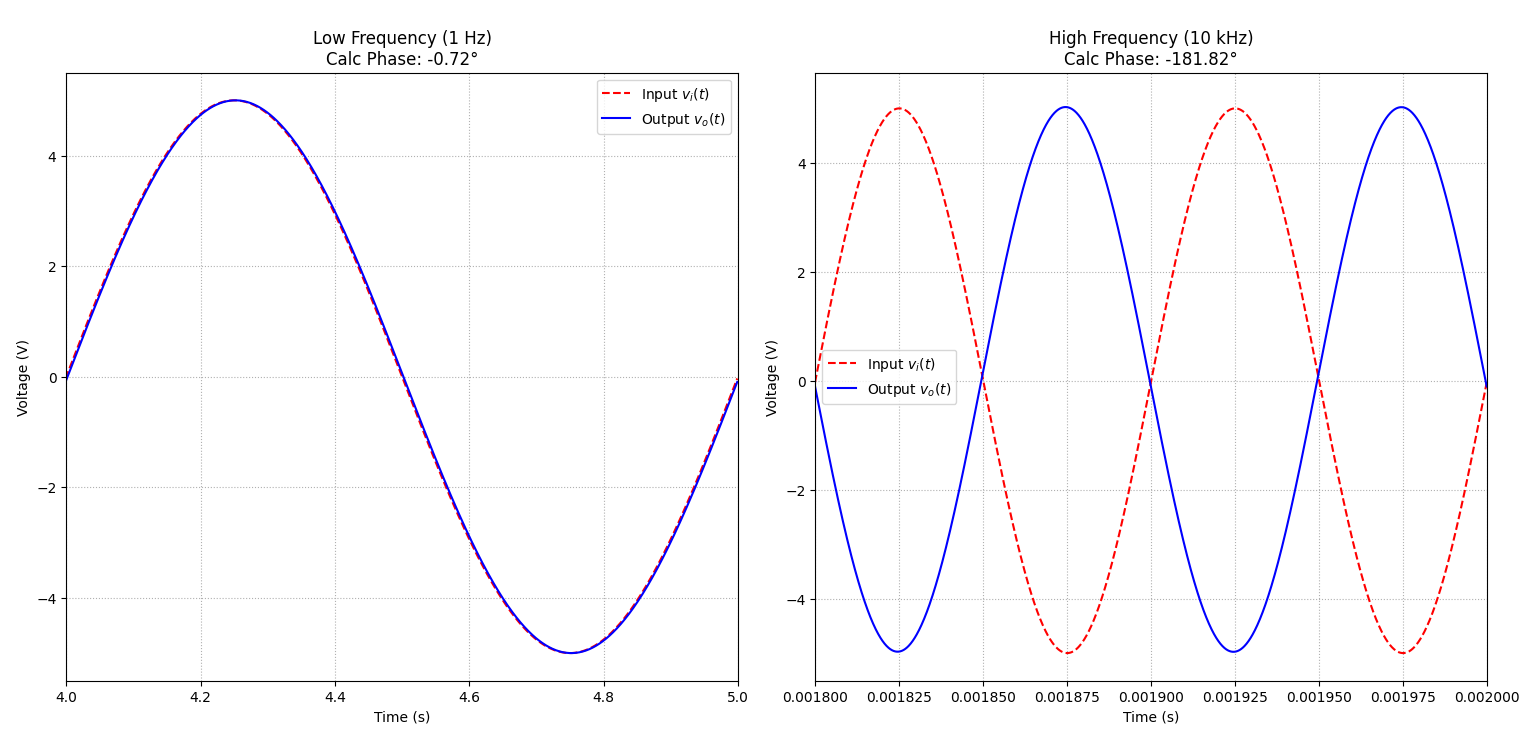
\includegraphics[width=\linewidth]{plot3.png}
    \caption{Plot}
    \label{fig:placeholder}
\end{figure}
    
\end{frame}

\begin{frame}[fragile]
\frametitle{Python Code for Plot}


\begin{mycode}
import numpy as np
import matplotlib.pyplot as plt

R = 1000 
C = 1e-6
RC = R * C

# 1. Create the time vector
t = np.linspace(-0.001, 0.005, 1000)
dt = t[1] - t[0] # Time step size

# 2. Define the Step Function u(t)
u = np.where(t >= 0, 1, 0)

# 3. Define the Continuous Exponential Part

h_continuous = (2/RC) * np.exp(-t/RC) * u


\end{mycode}

\end{frame}
\begin{frame}[fragile]
\frametitle{Python Code for Plot}
\begin{mycode}

# 4. Define the Delta Function numerically
delta = np.zeros_like(t)
delta[np.abs(t).argmin()] = 1/dt 

# 5. Combine into the final h(t)
h_final = -delta + h_continuous

# Plotting
plt.figure(figsize=(9, 6))
plt.plot(t, h_final, label=' $h(t)$ Calculation', color='blue', lw=2)

# Aesthetics
plt.axhline(0, color='black', lw=1)
plt.axvline(0, color='black', lw=1)

\end{mycode}

\end{frame}

\begin{frame}[fragile]
\frametitle{Python Code for Plot}
\begin{mycode}


plt.ylim(-1000, 2500) # Zoom in to see the behavior clearly
plt.title(r' Time-Domain Plot of $h(t) = -\delta(t) + \frac{2}{RC}e^{-t/RC}u(t)$')
plt.xlabel('Time (s)')
plt.ylabel('Amplitude')
plt.grid(True, linestyle=':', alpha=0.6)
plt.legend()
plt.show()
\end{mycode}

\end{frame}




\begin{frame}{Python plot}
    \begin{figure}
        \centering
        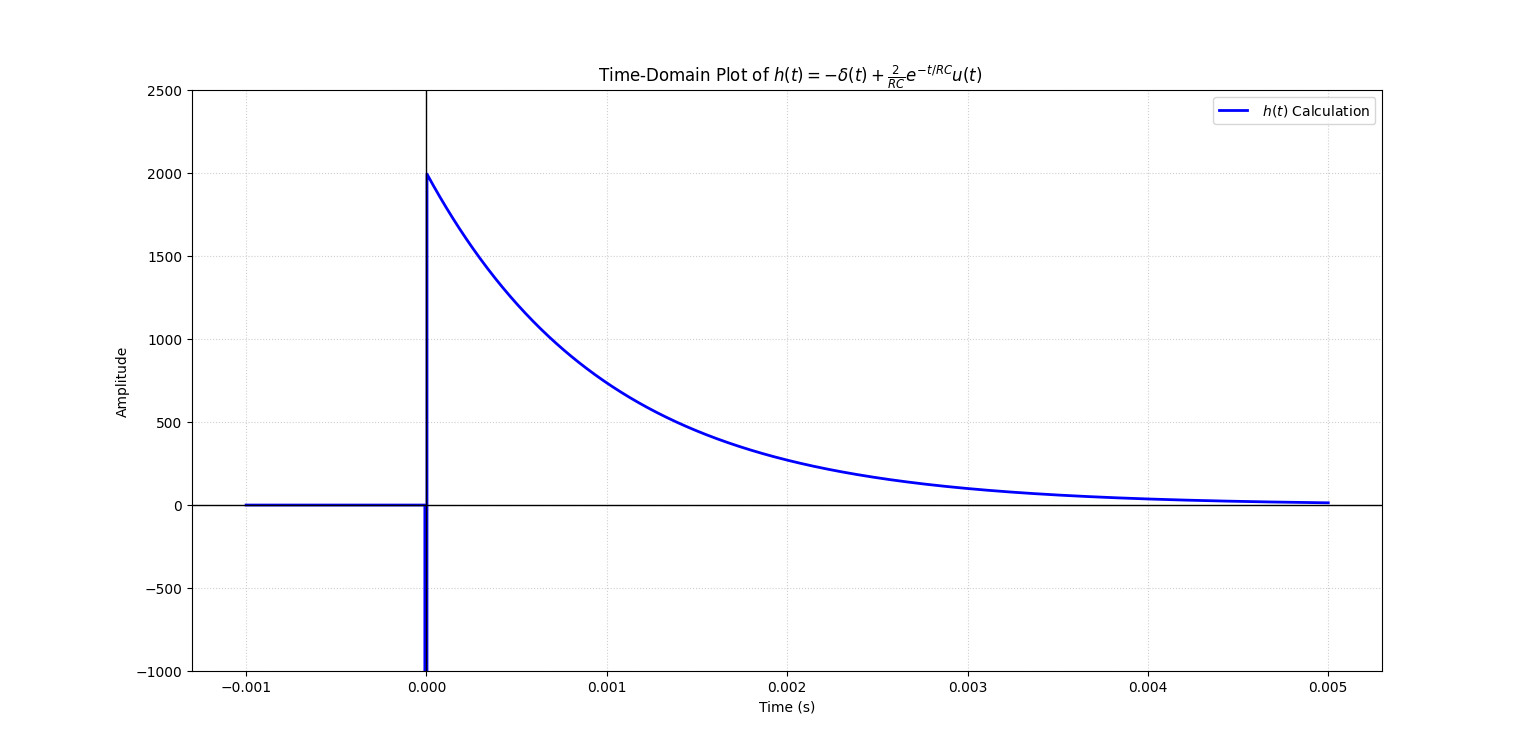
\includegraphics[width=\linewidth]{plot2.png}
        \caption{Plot}
        \label{fig:placeholder}
    \end{figure}
\end{frame}
\end{document}